\section{Experiments}\label{sec:experiments}

In this section, we report on experimental measurements illustrating the concrete improvements
in latency of PoEM as compared to Bitcoin. We implemented a stochastic simulation in 1500 lines of
Rust code\footnote{
    \ifanonymous
    The source code is available in the following anonymized repository:
    \url{https://anonymous.4open.science/r/anonymized-poem-simulations-A2FC}
\else
    The source code is available in the following repository:
    \url{https://github.com/commonprefix/poem/tree/main/simulation}
\fi
} and used Python's matplotlib
to plot the results comparing Bitcoin and PoEM.

We simulate various executions of Bitcoin and PoEM with different parameterizations.
In each simulated execution, we fix the block production rate $g$ (honest blocks produced per network delay $\Delta$),
the adversarial ratio $\beta$ (ratio of adversary's mining power divided by the total mining power),
and, for PoEM, also the bias parameter $\gamma$, and we
measure the latency of the system. The latency is defined as the time it takes for a new transaction
to become stable in the system (i.e., $k$-confirmed for a sufficiently large $k$).
The challenge is to measure the latency of the two
systems at the same \emph{security level}. As the two systems operate differently, simply
taking the same number of blocks (or work) does not constitute a fair comparison.

We measure the time needed from the moment an honest block is mined until
the first time any honest party considers the block \emph{stable}, and only for those blocks
which eventually do become stable.
We use the private mining attack as the adversarial strategy, which was
proven~\cite{eiar} to be the best possible attack against Bitcoin in the continuous-time model~\cite{bitcoin-made-simple}.
In a nutshell, in this strategy, the adversary mines blocks in private on her own chain, whereas the honest parties mine
their own blocktree, following the heaviest chain rule (in Bitcoin) or the most intrinsic work rule (in PoEM) respectively.
The adversary imposes a network delay of $\Delta$ on honest parties.
Our simulation begins with all honest parties and the adversary agreeing on a particular genesis block
$G$ with no premining having occurred. At that point, the adversary uses the private mining strategy
with the goal of conducting a double-spend in a block immediately following $G$.
For a particular execution simulation sample, we determine the \emph{safe} confirmation parameter $k$
that the honest parties \emph{should} have used to avoid this double-spend.
Whereas in our experiments, this confirmation parameter is determined retroactively,
in the real implementation, the confirmation parameter should be determined prospectively.

We simulate the adversary and the honest parties independently. On the one hand, the adversary mines blocks
in a chain without incurring any delay, and therefore without any forks. The adversary's block production rate is
$g\frac{\beta}{1 - \beta}$. On the other hand, the honest parties incur a network delay of $\Delta$ for each mined block,
and they mine blocks at a rate of $g$. Because of this delay, the blocks mined by the honest parties form a blocktree.

To save time, instead of wastefully simulating proof of work, we artificially simulate block production using a
continuous-time stochastic process.
We know that the time between the creation of two honest blocks is exponentially distributed
with rate $g$ (because the times of block creation form a Poisson point process~\cite{bitcoin-made-simple}).
Hence, we take multiple independent samples from $\exp(g)$ to get the interval between each successive honest block production event,
thereby giving rise to a Poisson process of honest block creations (even though these blocks may not necessarily be placed in a chain).
We simulate a similar independent Poisson process for the adversary
by sampling from $\exp(g\frac{\beta}{1 - \beta})$. These two stochastic processes produce the block creation times of the honest and
adversary parties, from which we can determine the blocktree that was constructed taking the delay into account.

In Bitcoin, the work of each block is equal to one,
whereas in PoEM, the work of a block is
distributed as $\gamma + \exp(\frac{1}{\ln2})$ (as we show in the Analysis section). Note that these biased exponential samples of \emph{work} are a different,
parallel process from the exponential samples of \emph{time intervals} between block creations.
Hence, in PoEM's case, we sample from $\gamma + \exp(\frac{1}{\ln2})$ to get the work
of each block in the execution. The creation time of each block and its work are enough to simulate the honest parties' execution
and determine the blocktree that was constructed.
The honest blocktree is computed as follows: We create a list of \emph{events} pertaining to either the creation of a new honest block,
or the arrival of the block to the rest of honest parties $\Delta$ later\footnote{Delaying all blocks by the maximum possible delay $\Delta$
was proven to be an optimal adversarial strategy~\cite{eiar}.}.
We sort these events in chronological order and process them one by one.
Throughout time, we maintain a single value indicating the cumulative work of the heaviest chain seen so far by all honest parties.
For every block, we also keep the cumulative work of the chain ending at that block.
At the block creation event, we compute the cumulative work associated with the block as the cumulative work of the
heaviest chain seen so far plus the work of the block (1 in Bitcoin, sampled in PoEM). At the block arrival event, we compare the
cumulative work of the chain ending at the arrival block with the cumulative work of the heaviest chain seen so
far\footnote{We make the usual~\cite{eiar} simplifying assumption that the number of mining parties $n \to \infty$, meaning
that each block is mined by a different party.}.
If it is heavier, we update our best cumulative work value. Every time we update the best cumulative work value,
we remember this cumulative work together with the creation timestamp associated with the block that caused the work to increase.

Then, independently we simulate the adversary's execution. Like in the honest execution, we sample from $\exp(g\frac{\beta}{1 - \beta})$
to get the interval between the time of successive adversarially produced blocks, where $g\frac{\beta}{1 - \beta}$ is the adversary's block production rate.
Then, similar to the honest simulation, we set the work of each block to $1$ in Bitcoin, and sample from $\gamma + \exp(\frac{1}{\ln2})$ to get the work of each block in PoEM.
Since the adversary has no network delay, all her blocks are chained in series.
Again, we maintain an association of timestamps and cumulative work values for every block.

Having simulated the honest and adversary executions, we can now determine the latency of the system (whether Bitcoin or PoEM).
To find this latency, we must find the minimum \emph{safe} confirmation parameter $k$ (where $k$ is denominated in \emph{amount of work} per block, as measured
by the respective system).
To do this, we determine the \emph{last} point in time when the adversary had a chain with more work than the honest parties,
and we record the work $k$ of the honest chain that first surpasses the adversary's chain immediately after.
For this execution, a confirmation parameter larger or equal to $k$ would safeguard the protocol from a Common Prefix violation.

To accurately calculate the latency of a given system parameterization $(g, \beta)$ -- and, for PoEM, also $\gamma$ -- we
simulate $100{,}000$ such executions and record the minimum safe confirmation
parameter $k$ for each execution. We wish to determine the value of $k$ that gives a specific
security level -- in our case, we want $90\%$ of the executions to be safe from a Common Prefix violation (i.e., $3.32$ bits of
security\footnote{While $-\lg_2(10\%) = 3.32$ bits of security are not enough for cryptographic security, we use this as a
reference to compare the latency of the two systems. On the contrary, our theoretical analysis shows that PoEM is secure with \emph{overwhelming} probability
in the security parameter $\kappa$.}).
Intuitively, using a common reference security level is what allows us to fairly compare these disparate systems.

In a nutshell, we set $k^*$ to be the minimum confirmation parameter that would safeguard $90\%$ of the executions against a Common Prefix violation.
To do this, we collect all the safe $k$ values of the $100{,}000$ Monte Carlo iterations into a list.
We take the $20\%$ highest percentile of the list and set $k^*$ to be the mean of these values (i.e., the \emph{expected shortfall}
at $20\%$, noting that the $90\%$ mark falls in the middle of the top $20\%$ percentile).

\begin{figure}[h]
    \centering
    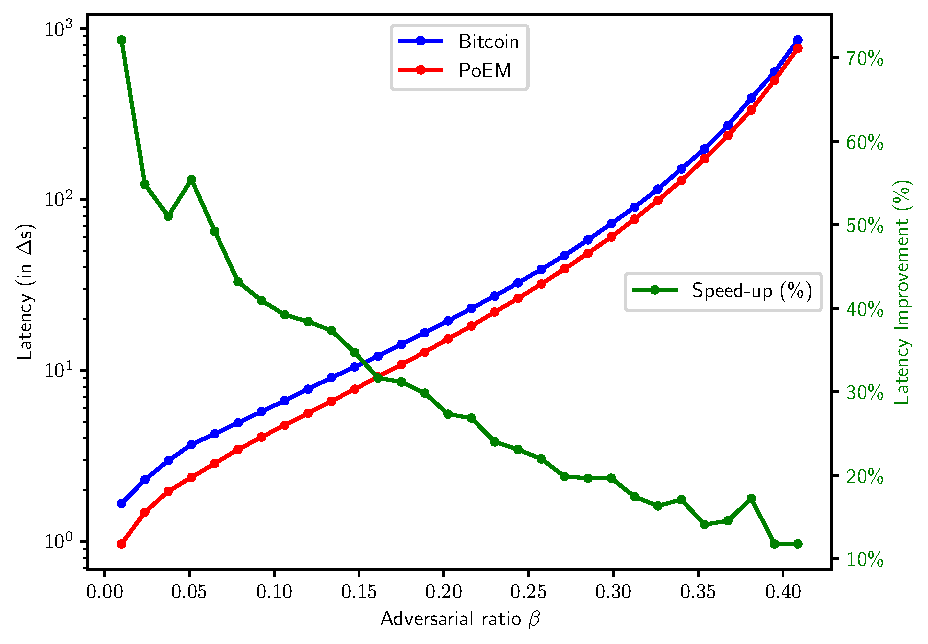
\includegraphics[width = 0.9\textwidth]{figures/bitcoin_vs_poem.pdf}

    \caption{Bitcoin vs PoEM latency (logarithmic scale) over different adversarial ratios $\beta$.
             The results were obtained by running 200 million simulations per point.
             For every value of the triplet $(\beta, g, \gamma)$, we perform
             $100{,}000$ Monte Carlo iterations and obtain the latency-optimal parameters
             $(g, \gamma)$ for which the latency is illustrated on the vertical axis.}
    \label{fig:bitcoin_vs_poem}
\end{figure}

The latency of the system is calculated as $d = \frac{k^*}{f}$, where $f$ is the average cumulative work increase rate for the honest chains.
The latency $d$ is the average time it takes to produce $k^*$ chained honest work in the system (both in Bitcoin and PoEM).
To acquire $f$, we calculate the honest cumulative work increase rate for each execution and take their average across all Monte Carlo iterations.
Namely, for each execution, we take the maximum honest cumulative work achieved during the execution's lifetime, and divide it by the time
at which it occurred.

We get the optimal system latency for $30$ different adversarial ratios $\beta$ ranging linearly from $0$ to $0.4$.
We explore the latency of the system for $50$ different block production rates $g$ increasing geometrically from $0.05$ to $85$ blocks per network delay.
For PoEM, we explore $40$ different bias parameters $\gamma$ starting at $0$ and then ranging geometrically from $0.01$ to $20$.
For each tuple $(\beta, g, \gamma)$, we run the $100{,}000$ Monte Carlo iterations to obtain the
confirmation delay that achieves $90\%$ security (in the expected shortfall sense), and find the minimum delay across all configurations $(g, \gamma)$ (for PoEM)
and $g$ (for Bitcoin) for each $\beta$.
These optimal latencies are illustrated in Figure~\ref{fig:bitcoin_vs_poem}.
For each point in the plot, we ran $100{,}000 \times 50 \times 40 = 200{,}000{,}000$ PoEM simulations
and $100{,}000 \times 50 = 5{,}000{,}000$ Bitcoin simulations,
for a total of $6.15$ billion simulation runs across all points in the plot.

% TODO: Explain the following aspects of the experimental methodology:
% 1) Talk about the initial sampling of the adversarial execution and the scaling with $\beta$ retroactively
% 2) infinite values not taken into account
% 3) lifetime of simulations
% 4) Quantization

We observe that PoEM outperforms Bitcoin in terms of latency across all adversarial ratios $\beta$.
For small values of $\beta$, PoEM has as much as $70\%$ faster confirmation than Bitcoin.
The speedup decreases as $\beta$ increases, but PoEM still outperforms Bitcoin by $11.7\%$ for adversarial ratios around $0.4$.
For small adversarial presence, the block production rate $g$ of PoEM can be safely increased much more than in Bitcoin.
This is illustrated in Figure~\ref{fig:g}.
It is for these larger values of $g$ that PoEM truly shines, utilizing more effectively the work of the
forks that appear in the honest blocktree (Figure~\ref{fig:poem-wasted-work}).

% TODO: fix the fonts that are sans-serif in these figures
% TODO: make all figures readable in grayscale
\begin{figure}[h]
    \centering
    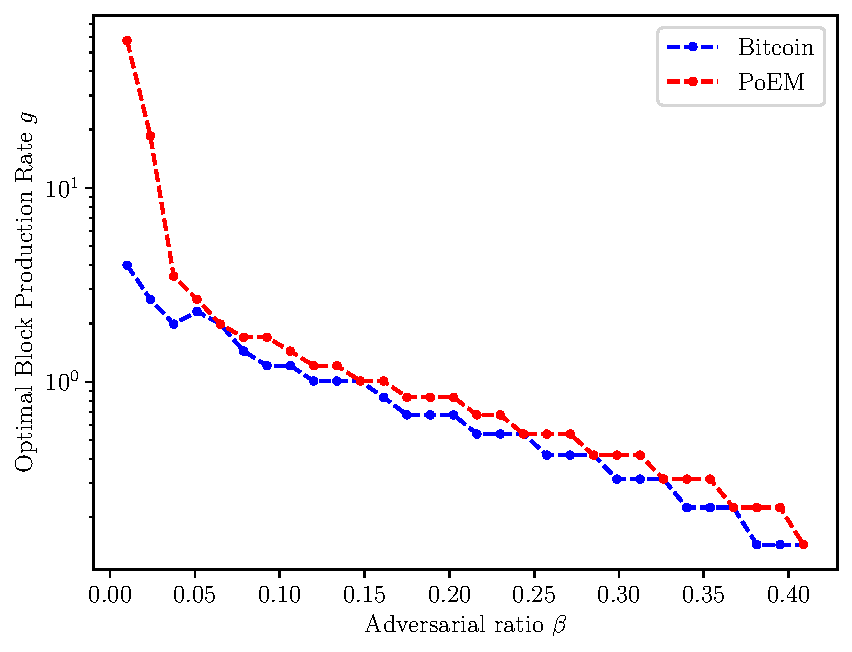
\includegraphics[width = 0.8\textwidth]{figures/g.pdf}

    \caption{Bitcoin vs PoEM optimal block production rate $g$ (logarithmic scale) over different adversarial ratios $\beta$.
             The results were obtained by running $100{,}000$ Monte Carlo iterations for each parametrization triplet
             $(\beta, g, \gamma)$, for a total of $200{,}000{,}000$ simulations per point.}
    \label{fig:g}
\end{figure}

We note some limitations of our experimental methodology. Firstly, the private attack has been proven optimal
for Bitcoin only, and not for PoEM, but in our experiments we have used the same attack for both protocols.
Secondly, the optimality of the private attack previously proven~\cite{eiar} is a reduction illustrating
that, for a given resilience $\beta$, if the private attack is not possible, then no attack is possible.
In our experiments, we obtain a safe confirmation parameter $k$ against the private mining attack,
but this confirmation parameter has not been shown to be safe against other attacks, even though the private
mining attack is optimal when it pertains to resilience.
Lastly, there is a discrepancy between the continuous-time model used in our experimental simulations
and the discrete-time model used in our theoretical analysis.

\noindent
\textbf{Real-world Deployment.}
In addition to the above simulations,
we have implemented and deployed\footnote{
    \ifanonymous
        The source code is available in the following anonymized repository:
        \url{https://anonymous.4open.science/r/go-quai-3182}
    \else
        The source code can be found at
        \url{https://github.com/dominant-strategies/go-quai/releases/tag/v0.28.2}
    \fi
} PoEM in a real-world permissionless peer-to-peer
setting.
The deployment is on a testnet that has been continuously operating for
four months. During this period, the network generated 7.5 million blocks
and 500 million transactions
with participation from 2000 miners from the community, maintaining an
average hash rate of 50GH/s using ProgPoW~\cite{progpow}.
The miners computed 518 petahashes in 4 months,
with the difficulty ($\frac{2^{256}}{T}$)
varying between 18 billion and 790 billion.
